
\subsubsection{\Hbb combination}
\label{sec:vbf-hbbcomb}

In 2018, \Hbb is observed at the ATLAS experiment \cite{VHPaper} confirming the Higgs to quark Yukawa coupling. Three separate \Hbb production modes: VH, ttH and VBF including both Run I and Run II data are combined for a measurement. The 7\TeV data and 8\TeV data have luminosity of $4.7\ifb$ and $20.3\ifb$ respectively. The 13\TeV analyses use data with luminosity ranging from $24.5-79.8\ifb$. This combination measured observed signal strength to be $\mu_{\Hbb}= 1.01 \pm 0.20 = 1.01 \pm 0.12\text{(stat.)}^{+0.16}_{-0.15}\text{(syst.)}$ with a $5\sigma$ significance.


\begin{figure}[htbp]
  \centering
 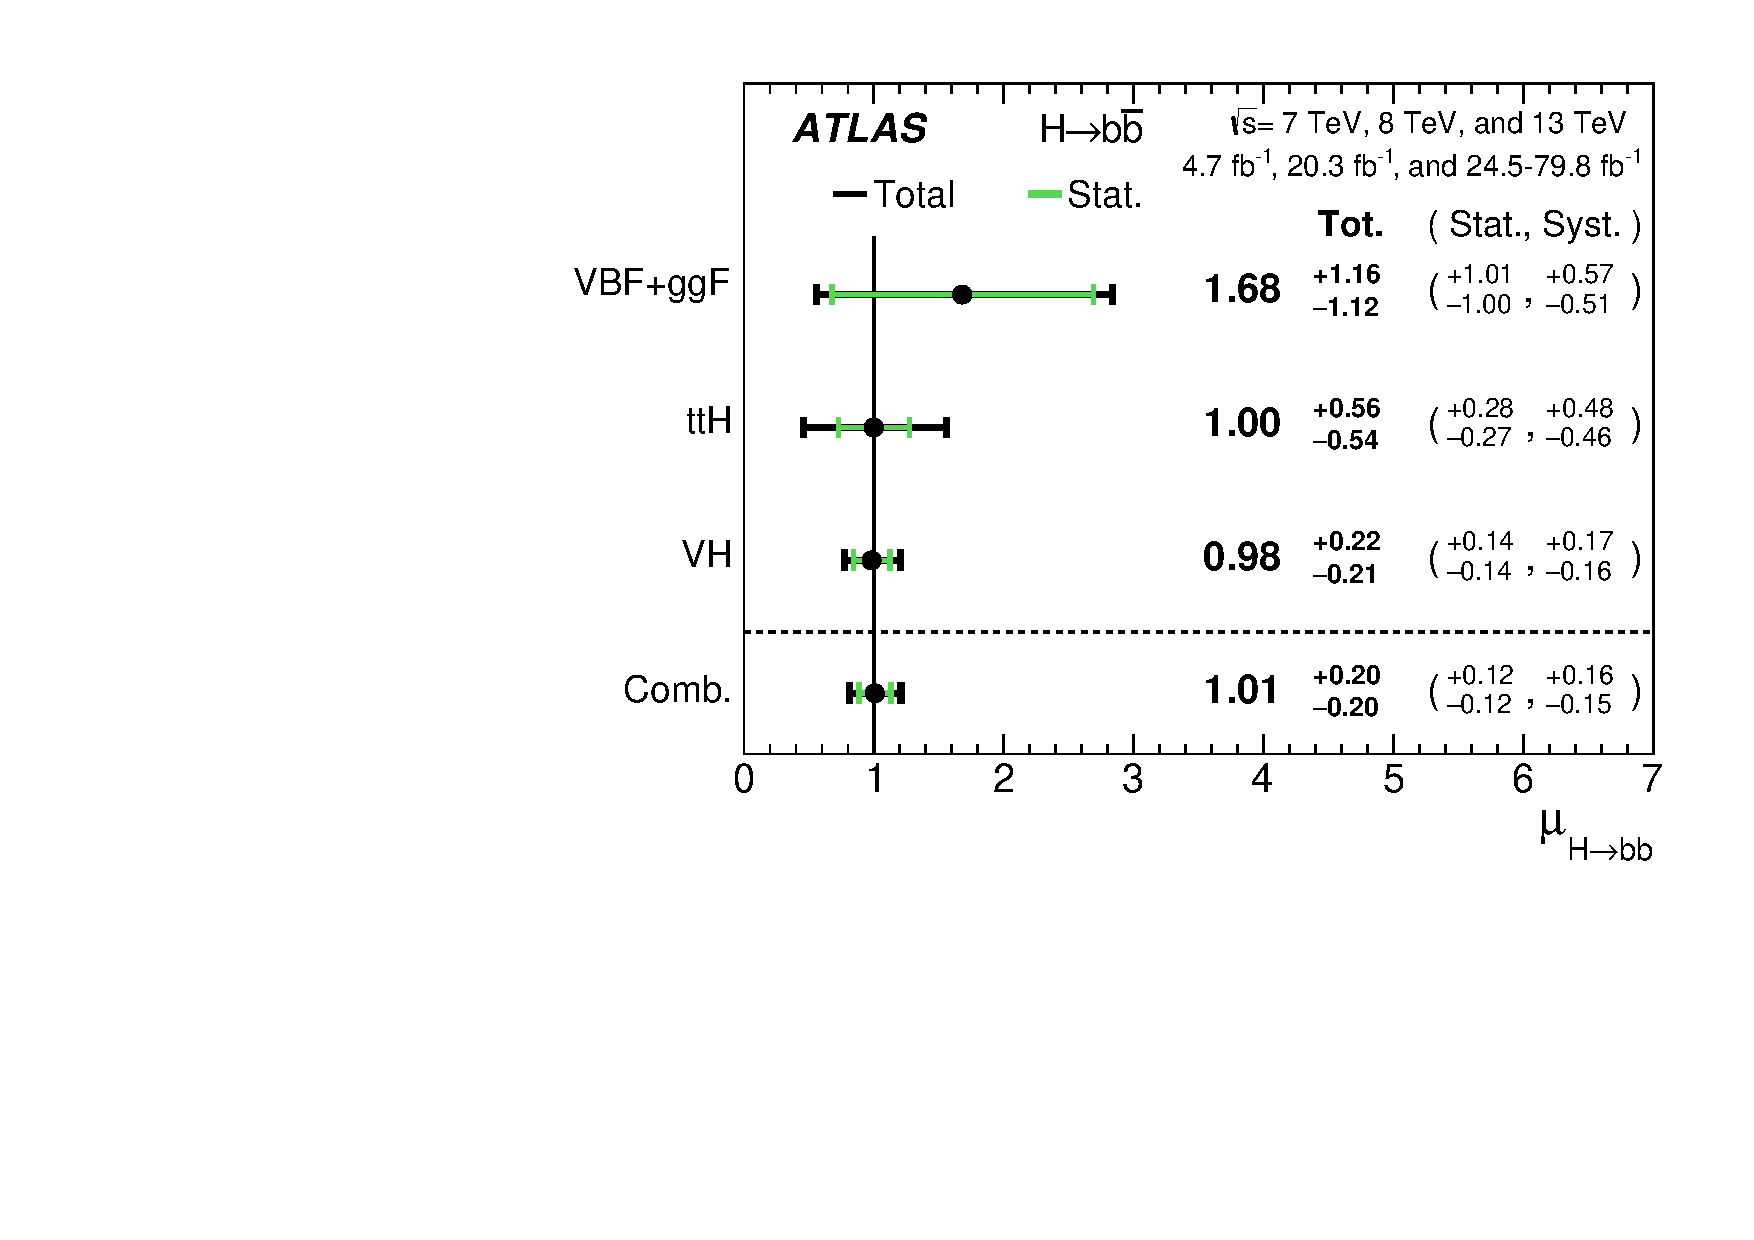
\includegraphics[width=0.8\textwidth]{figures/VBF/HbbComb.pdf}
 \caption{The fitted Higgs boson signal strength for the \Hbb combination. The combination includes 7\TeV, 8\TeV and 13\TeV data of VH, ttH and VBF analyses. Probability of signal strength compatibility of individual channel signal strengths is 83\%.}
  \label{fig:vbf-combination-hbb}
\end{figure}



%\subsubsection{Higgs combination}
%\label{sec:vbf-higgscomb}
% To be filled in.
